% \documentclass[PhD]{nitgoathesis}
%\documentclass[MTech]{nitgoathesis}
\documentclass[BTech]{nitgoathesis}
\usepackage{times}
 \usepackage{t1enc}

\usepackage{graphicx}
\usepackage{epstopdf}
%\usepackage[hypertex]{hyperref} % hyperlinks for references.
\usepackage{amsmath} % easier math formulae, align, subequations \ldots
\usepackage{url}
\usepackage{slashbox}
\usepackage{color}
\definecolor{bg_text}{rgb}{0.8,0.8,0.8}
\definecolor{mygreen}{rgb}{0,0.6,0}

\usepackage{listings}
\lstset{
numbers=left,
language={},
breaklines=true,
basicstyle=\ttfamily\footnotesize,
backgroundcolor=\color{bg_text}
}


\begin{document}


%%%%%%%%%%%%%%%%%%%%%%%%%%%%%%%%%%%%%%%%%%%%%%%%%%%%%%%%%%%%%%%%%%%%%%
% Title page

\title{Automatic Text Summarization}


\author{  Vighnesh Birodkar  (10CSE008) \vskip 1mm
 Dhruv Jawali  (10CSE009)}

\date{APRIL 2014}
\department{COMPUTER SCIENCE AND ENGINEERING}

%\nocite{*}
\maketitle

%%%%%%%%%%%%%%%%%%%%%%%%%%%%%%%%%%%%%%%%%%%%%%%%%%%%%%%%%%%%%%%%%%%%%%
% Certificate
\certificate

\vspace*{0.5in}

\noindent This is to certify that the work contained in this Dissertation entitled ``Automatic Text Summarization'' 
submitted by the group members Mr. Vighnesh Birodkar (Roll. No: 10CSE008)  and Mr. Dhruv Jawali, (Roll. No: 10CSE009) to the 
Department of Computer Science and Engineering, National Institute of Technology Goa, for the partial fulfilment of the requirements for 
the degree of Bachelor of Technology in Computer Science and Engineering. They have carried out their research work under my 
supervision. This work has not been submitted else- where for the award of any other degree or diploma.\newline
\noindent The Dissertation, in my opinion, has reached the standard fulfilling of the requirements for the degree of Bachelor of 
Technology in Computer Science and Engineering in accordance with the regulations of the Institute.

\vspace*{1.5in}

\begin{singlespacing}
\hspace*{2.8in}
\parbox{3in}{
\noindent {Mrs. Veena T.} \\
\noindent Assistant Professor \\ 
\noindent Computer Science and Engineering Department \\
\noindent National Institute of Technology Goa-403401\\
\noindent  \\
} 
% \hspace*{2.8in}
% \parbox{3in}{
% \noindent {Name of the Guide} \\
% \noindent Designation \\ 
% \noindent Department Name \\
% \noindent National Institute of Technology Goa-403401\\
% \noindent  \\
% } 
\end{singlespacing}



%%%%%%%%%%%%%%%%%%%%%%%%%%%%%%%%%%%%%%%%%%%%%%%%%%%%%%%%%%%%%%%%%%%%%%
% Acknowledgements
\acknowledgements

We  would like to express our gratitude to our respected Director Dr. G.R.C Reddy for his constant motivation and for providing excellent infrastructure. 
We wish to thank and express our sincere gratitude to the Computer Science Department of NIT Goa for motivating us to pursue Text Summarization. In particular, we thank our guide Mrs. Veena T for her constant support and encouragement towards the completion of this project.  Her guidance has been a source of inspiration to both of us.
Last but not the least we would like to thank our parents and friends for their timely support, constant advice and the healthy criticism that made this project a success.

%%%%%%%%%%%%%%%%%%%%%%%%%%%%%%%%%%%%%%%%%%%%%%%%%%%%%%%%%%%%%%%%%%%%%%
% Abstract

\abstract
With the advent of the Internet, storing and sharing of information became much easier, though in recent years \emph{information explosion} has become a problem. This has motivated research into Automated Text Summarization techniques, which involves generating a concise, coherent summary of input document(s) with minimal loss of information. Many diverse approaches have been used in the past to attack this problem, including document statistics, Machine Learning, document structure etc. Modelling Text Summarization as a Machine Learning Problem offers interesting advantages such as the ability to capture the nuances of extracting relevant information from a document simply by specifying a set of local and global sentence features. In this project, we explore a novel way to use human generated summaries to train a Regression Model in order to perform Extractive Summarization. We evaluate our method against three different types of documents, and observe that the quality of summaries generated is sensitive to the type of document(s) used for training.
% \noindent KEYWORDS: \hspace*{0.5em} \parbox[t]{4.4in}{\LaTeX ; Thesis;
%   Style files; Format.}

% \vspace*{24pt}
% 

\pagebreak

%%%%%%%%%%%%%%%%%%%%%%%%%%%%%%%%%%%%%%%%%%%%%%%%%%%%%%%%%%%%%%%%%
% Table of contents etc.

\begin{singlespace}
\tableofcontents
\thispagestyle{empty}


\listoffigures
\addcontentsline{toc}{chapter}{List of Figures}
\end{singlespace}


%%%%%%%%%%%%%%%%%%%%%%%%%%%%%%%%%%%%%%%%%%%%%%%%%%%%%%%%%%%%%%%%%%%%%%
% Abbreviations

% The main text will follow from this point so set the page numbering
% to arabic from here on.
\pagenumbering{arabic}


%%%%%%%%%%%%%%%%%%%%%%%%%%%%%%%%%%%%%%%%%%%%%%%%%%
% Introduction.


\chapter{Introduction}
\emph{Information Explosion} \cite{fshock} refers to the rapid increase in the amount of published information or data, and the effects of this abundance. The Internet now consists of at least 4.3 billion web pages \cite{websize}. With each passing day, this number increases. Storing, interpreting and maintaining the ever increasing amount of information on the internet is going to be a challenge in the near future.
\par
Computers are ideal for storing and manipulating data, but lack the means to interpret it. Formally defining grammars for human languages is not possible, since the meanings of words are sensitive to the context. As a result, in the present scenario, the task of understanding and interpreting text data is a task primarily limitied to human subjects. Although data on the internet keeps growing exponentially, the same is neither true for the people overseeing this growth, nor for the people looking to access this information; for example, the flood of technical reviews when a new product is launched. Potential customers might have to sift through the dozens of review websites, looking for salient points in each review. It would be much easier if the information on these websites could be collected and compiled into a single, coherent document.
\par
Until computers are capable of interpreting human languages, humans must be kept in the loop. We need a system to limit the data the humans have to oversee, without omitting important facts. This is acheieved through \emph{Text Summarization Techniques}.
\par

With the current state-of-the-art in Natural Language Processing (NLP), it highly difficult, if not impossible, to design a system which derives semantic information from a text document. Hence, current text summarization techniques rely on statistical measures of importance, combined with heuristics, to assign scores to sentences within the document to create summaries. Some techniques based on forming new sentences, rather than just extracting sentences from the given set of documents, take advantage of parts-of-speech tagging, and identify semantic structure within documents. These structures, however, are limited to the type of documents being summarized, and are subject to the limitations faced by the NLP techniques used to describe them.
\par

An interesting way to look at the Text Summarization Problem is to pose it as a Machine Learning Problem. Using the statistical measures defined to order sentences in other extractive techniques, we model the importance of a sentence (a measure of whether it should appear in the summary or not) as a combination of these measures, and learn the weights assigned to them from human generated summaries. A regression technique is used for training, and a set of documents with summaries written by humans are used to generate scores for each sentence in the document.  In this project, we develop a novel way to generate scores for sentences in a document based on abstractive summaries written by humans, which are used to train a regression model. This model can then be used to generate extractive summaries. Evaluation of these summaries is done by generating Recall Oriented Understudy for Gist Evaluation (ROUGE) scores.
\chapter{Automatic Text Summarization}
Research in automated text summarization techniques has been ongoing for nearly half of the last century, during which time the problem has been addressed with varying perspectives and paradigms. Most of the community agrees on the following points as to what a summary should be \cite{survey}:
\begin{itemize}
\item Summaries may be produced from a single document or multiple documents.
\item Summaries should preserve important information.
\item Summaries should be short.


\end{itemize}
However, a more elaborative definition can be prohibitive, since the approaches taken towards text summarization often differ in the manner of their problem formulation \cite{survey}. 
\section{Terminology}
\begin{itemize}


\item Extraction: Selection of important sentences or sections from a set of documents, and reproducing them verbatim to create a summary of their salient points.
\item Abstraction: Extracting information from a set of documents and presenting it in a new way; generally involves using Natural Language Generation techniques.
\item Fusion: Combination of extracted sentences into a coherent summary, using Natural Language Processing techniques.
\item Compression: Keeping important points from a set of documents, by eliminating redundancies. \cite{meadsystem}
\end{itemize}
The following example illustrates extractive and abstractive summaries.\\
\newpage
{\noindent \large \underline{Example}} 

\begin{lstlisting}[numbers=none]
Tardigrade.
Tardigrades are 0.5 mm long water dwelling animals.
They are segmented animals with 8 legs.
Tardigrades can live for 10 years without food are water.
They can even survive the vacuum of space.
They have survived all 5 mass extinctions on earth.
\end{lstlisting}
\vspace{1.2em}
{\large Extractive Summary}
\begin{lstlisting}[numbers=none]
Tardigrades are 0.5mm long water dwelling animals.
Tardigrades can live for 10 years without food are water
\end{lstlisting}
\vspace{1.2em}
{\large Abstractive Summary}
\begin{lstlisting}[numbers=none]
Tardigrades are 0.5 water dwelling creatures with 4 segments 
and 8 legs.
They can libe without food and water for 10 years and even 
survive the vacuum of space.
\end{lstlisting}
As we can see from the example, abstractive summaries are able to represent more of the information concisely. But current abstractive summarization techniques are a long way from the human ability to do so.


\section{Evolution of Text Summarization}
The information contained in a document is not uniform; there exist many descriptive, redundant sentences, and relatively few sentences which convey information. The challenge faced while summarization is to identify and reproduce the important information while getting rid of the redundant parts. Text Summarization can broadly be classified under the following two types:
\par
\begin{itemize}
\item Single Document Summarization: A single, complete document has to be summarized. Extractive techniques from an Information Retrieval perspective has been explored in depth for Single Document Summarization.
\item Multi-Document Summarization: Multiple documents, containing salient and often conflicting views about the various themes in the documents need to be brought together to represent a coherent summary.
\end{itemize}
We now describe how Text Summariztion has evolved over the years, beginning with Single Document Summarization.
\subsection{Single Document Summarization}
\subsubsection{Early Work}
The earliest approaches taken for Text Summarization were based on using features like word and phrase frequency \cite{lun}, position of sentences in text \cite{bax} and key phrases from text \cite{edm}. These seminal contributions have gone a long way to establish that a statistical approach to summarization can be quite effective. The idea of ranking sentences by assigning them significance factors comes from \cite{lun}, which has since inspired many similar techniques of extractive summarization. The author of \cite{edm} has been credited with the development of a typical extractive summarization system; he used the features proposed in \cite{lun} and \cite{bax} along with two of his own features ie. presence of cue words in a sentence, and skeletal structure of the document, and defined the significance as a weighted sum of these features. He calculated these weights manually, and the results were compliant with around 44\% of manual extracts.

\subsubsection{Machine Learning Methods}

In the 1990s, as Machine Learning methods in NLP gained popularity, many research papers appeared which employed statistical methods to produce summaries. The idea put forward in \cite{edm} was used, and the weights for various features were learned using machine learning techniques.
\par
\cite{kup} used a naive-Bayes classifier (making the assumption that features were independent) to learn weights, and extended the idea of \cite{edm} by adding two more features - sentence length and presence of uppercase words. The method was evaluated against technical documents, where the authors selected sentences from the document mapping to the abstract manually, and compared these with the summary generated by their system. It was observed that the sentence position, cue words and sentence length features were most significant, and a system comprising only these performed best.
\cite{aone} made use of a naive-Bayes classifier as well, though with richer features, such as tf-idf scores. This was mostly evaluated against newswire corpora.

\par
\cite{linhovy} extended the idea in \cite{bax} to improve upon the definition of sentence position in text, to accommodate for the varying discourse structures of text over different domains. In further work, \cite{lin} used decision trees to model sentence extraction, instead of the naive-Bayes classifier (breaking away from the assumption of independent features), and experimented with a lot of features. The publicly available documents provided by the TIPSTER-SUMMAC evaluations was used for this work.

\par
\cite{conory} modeled the problem of sentence extraction using a hidden-Markov model, which captures local dependencies between sentences. Only three features were used - sentence position, number of terms, and likeliness of the sentence terms given the document terms. The summaries produced were evaluated against human generated summaries.

\par
\cite{osb} showed that a log-linear model produced better results than a naive-Bayes model, since feature independence cannot be assumed. This was shown to be true empirically.
In response to Document Understand Conference's (DUC) task of creating a 100-word summary of news articles, \cite{svore} put forward an algorithm based on neural networks and usage of third party datasets for extractive summarization. This method out-performed the baseline set by DUC with statistical significance. To do this, the authors made use of 1365 news articles with human generated summaries from CNN.com. Since the human generated summaries were not verbatim, ROUGE-1 scores \cite{lin} were used to to score sentences of the summaries against each sentence as a similarity measure. These were used as soft labels during the training phase. A similar idea is used in our project to learn from human generated summaries.

\subsubsection{Natural Langauge Processing Methods}
Natural language Analysis methods do not attempt to solve summarization through machine learning methods; instead, they develop heuristics based on the document’s discourse structure.
\par

\cite{barz} used linguistic analysis to define lexical chains: a sequence of related words in a text spanning short or long distances. Their method first performed text segmentation, followed by lexical chain extraction and finally, used strong lexical chains to extract sentences. This achieved a middle ground between using semantic structure of text and using word statistics for extraction, as seen in \cite{mck} and \cite{lun} respectively.
\par
In related work, \cite{ono} used a computational model to extract the discourse rhetorical structure of documents written in Japanese. This was done using a series of NLP steps: sentence analysis, rhetorical relation extraction, segmentation, candidate generation and preference judgement \cite{survey}. Results were quite satisfying, since important key sentence coverage was 74\%. 
\par
\cite{marc} used a novel approach involving Rhetorical Structure Theory (RST), which separates nucleus segments of text from satellite segments. The author makes the empirical observation that the nucleus segments express more important concepts than the satellites, though relation creates a tree like structure (the discourse tree). Extraction would then involve traversing this tree to decide which sentences are related and which ones should be included in the summary.

\subsection{Multi-Document Summarization}
Multi-document summarization gained popularity since the mid 1990s, finding applications in summarization of news articles, reviews etc. Many web-based news clustering systems were inspired by this research, such as Google news. These documents are characterized by their redundancy of information, as well as conflicting views. The challenges involve dealing with novelty, conflicts and producing a coherent and complete summary from the same.
\par
This field was pioneered by the NLP group at Columbia University \cite{mck}, where a summarization system called SUMMONS was developed. This is historically the first multi-document summarization system. Many approaches based on sentence similarity have been used; for example, clustering sentences which share a common theme and selecting one sentence which best represents the cluster \cite{mck}\cite{mead}. Other approaches include creating composite sentences from sentence clusters \cite{barz} and selecting sentences only if they contain some new information, using maximal marginal relevance \cite{carb}.
\par
Initially, claims were made that extractive systems would not be effective for multi-document summarization \cite{mck}\cite{mandall}. However, extractive systems like \cite{mead} achieved good performance in large scale news article summarization. This is probably due to a difference in the goals of these systems; some systems focus on form within strict domains, ie. producing a coherent summary using semantically correct, generated sentences, and thus rely on natural language generation techniques (SUMMONS). Others focus on more general domains, conforming to the Information Retrieval paradigm, with a focus on content rather than form (MEAD). Such systems are appealing since they do not rely on natural language generation, remaining domain independent and scalable.

\subsection{Abstractive Techniques}
Abstractive Text Summarization involves text segmentation and information extraction, which is then supplied to a Natural Language Generator. As mentioned before, such methods have narrow focus and need to be tuned according to discourse structure.
SUMMONS \cite{mck} is a notable example.
\par
OPINOSIS \cite{opn} is another technique which produces summaries for highly redundant opinions. 
\pagebreak
\chapter{A Machine Learning approach to Summarization}
Extractive summarization involves assigning an order to important sentences within the document. We need to separate the semantically important sentences from the unrelated or redundant sentences in the document. Using a combination of linguistic and statistical analysis techniques has proven effective in the past. When sentences are scored based on a set of features which capture their linguistic and statistical characteristics, it is often unclear how these features relate to each other. 
\par
\emph{Machine Learning} techniques can help "learn" these relationships to produce good summaries. A summarizing system can be trained to optimize a function of the document feature statistics depending on the context. This optimization relies on a training data set, which helps capture the relevant relationships. Ideally, a training sample should contain a document and an ordering of it's sentences, along with score values. However, purely extractive summaries are difficult to find, the system will have to be trained on abstractive summaries. The conversion from an abstractive to an extractive summary is an important step, since the training of the machine depends on it. Typical training data might include reviews and conclusions, papers and abstracts or movie plots and synopsis.
\par
To begin with, we represent each sentence in a given document as a vector. Each component of this vector represents a global or local feature of a sentence. The significance of a sentence in the a summary is a function of this vector. In fact, it is a weighted sum of the components of this vector ie. $f(v_i, v_j, v_k)$ where $v_i, v_j, v_k$ are the feature vectors. The weights of each component is what defines the function, which can be "learned" using regression, in our case, Support Vector Regression. 
\par
Finding a training dataset large enough to capture the feature space is a challenge while using Machine learning techniques. The results produced by a trained machine is very sensitive to the training data. Appropriate generation of training datasets is thus quite important. We use a measure called \emph{importance} to assign scores to sentences in a training document based on the human generated summaries. This is basically a measure of how similar each document sentence is to each summary sentence. Once the training data is obtained, we train a Support Vector Regression Model, which helps us predict the scores for the sentences in new documents, which are finally used to obtain the summary. \\
The approach we use is as follows :\\
\noindent{
\textbf{ Training Phase }
	\begin{itemize}
		\item Represent each sentence as a vector of features.
		\item Given a document and it's abstractive summary compute \emph{importance} of each sentence.
		\item Train a Regression Model to approximate the \emph{importance} of a sentence given it's feature vector.
	\end{itemize}
}
\noindent{
\textbf{ Prediction Phase }
	\begin{itemize}
		\item Represent each sentence as a vector of features.
		\item Used the train model to compute the \emph{importance} of a sentence.
		\item Order sentences by their \emph{importance} for the summary.
	\end{itemize}
}
To clarify how this approach is implemented, the following sections describe each measure and features we make use of.

\section{Definitions}
\textbf{\textit{Sentence}} $S$ is sequence of words $(w_1, w_2, ...... w_m )$ where $m$ is the number of words in the sentence. Length of a \textbf{\textit{Sentence}} $S$ is also abbrivated by the notation $|S|$ . Words are compared in a case-insensitive manner. Punctutations in sentences are not considered.\\

\textbf{\textit{Document}} $D$ is a sequence of \emph{Sentences} $(S_1, S_2, ......... S_n)$ where $n$ is the number of sentences in the document. Length of a \textbf{\textit{Document}} is also abbrivated by the notation $|D|$. \\

\textbf{\textit{Similarity}}\cite{textrank} between any two sentences $S_i$ and $S_j$ is defined as 
\begin{align}
 Similarity(S_i,S_j) =  { \cfrac{ |\{w_k | w_k \in S_i \&w_k \in S_j\}| }{log(|S_i|) + log(|S_j|)} }
\end{align}
An important thing to note here is that for two sentences which are mostly similar, the numerator in the expression for \emph{Similarity} increases linearly while the denominator increases logarithmically. Thus, larger sentences in the document matching larger sentences in the  summary get more significance.

\section{Sentence Features}
To be able to apply a regression technique we need to express each sentence as vector. This vector needs to capture the local as well as global significance of the sentence. For our purpose we have used the following 3 features.

\subsection{Text Rank Score}
To compute Text Rank Scores \cite{textrank} we model each sentence as a vertex in a graph. The Text Rank graph is completely connected, i.e. there is an edge connecting every two pairs of sentences. For a Document $D$, the weight between any two sentences is defined as 
\begin{align}
W( V_i,V_j) = W_{ij} = Similarity(S_i,S_j)
\end{align}

where $S_i,S_j \in D$  and $V_i,V_j$ are vertices corresponding to sentences $S_i,S_j$.\\
\\
The score for each sentence is computed as follows : 
\begin{align}
TR(V_i) = (1 - d)\ +\ d*\sum\limits_{V_j \in Adj(V_i)} \frac{W_{ji}}{\sum\limits_{V_k \in Adj(V_j)} W_{jk}} \times TR(V_j)
\end{align}
where $V_i$ is the vertex corresponding to Sentences $S_i$ in Document $D$, $TR(V_i)$ is the TextRank Score of $V_i$ and $Adj(V_i)$ is the set of vertices adjacent to $V_i$. $0 < d < 1$ is the damping factor and is set to $0.85$ \cite{brin}. The scores are computed repetedly till the algorithm converges. Convergence in this case is when the total update in scores over the entire graph, falls below a certain threshold. High \emph{Text Rank Score} implies that a sentence is talking about concepts which are being discussed elsewhere in the document. A sentence gets votes from other sentences, but votes from sentences having more score are more significant.\\
\par
{\noindent \large \underline{Example}} 
\begin{lstlisting}
Batman - The Dark Knight.
Batman is a superhero created by DC Comics.
He strives in Gotham city to prevent crime.
Gotham city is a corrupts metropolis swarmed by criminals.
Batman in real life is Bruce Wayne.
He is a multi-millionare owner of Wayne Corp.
His gadgets and vehicles are products of Wayne Corp.
Batman has no super human capabilities.
He relies darkness and stelath for advantage.
Hence he is often called the Dark Knight.
Batman is commited ridding Gotham of crime.
\end{lstlisting}  

The sum of magnitudes of the change in the score of each vertex keeps decreasing per iteration. The plot of Text Rank scores for the above example can be seen in Figure ~\ref{fig:tr}.We can see that Sentence 6 and Sentence 11 get high Text Rank scores because they talk about Wayne Corp and Gotham, which are also talked about elsewhere.The decreasing magnitudes of error per iteration can be observed in Figure ~\ref{fig:error}.

\begin{figure}[h!]
  \centering
    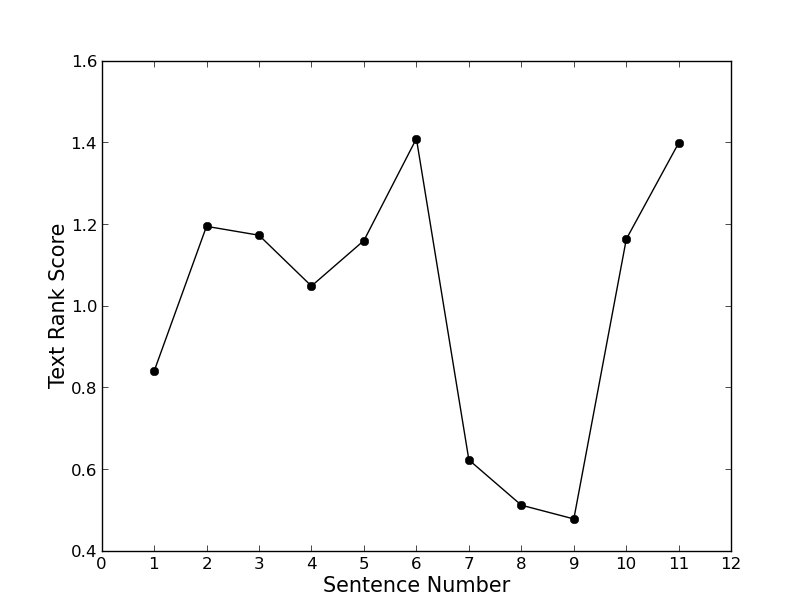
\includegraphics[width=.8\textwidth]{images/tr}
    \caption{A plot of Text Rank Scores }
    \label{fig:tr}
\end{figure}

\pagebreak
\begin{figure}[h!]
  \centering
    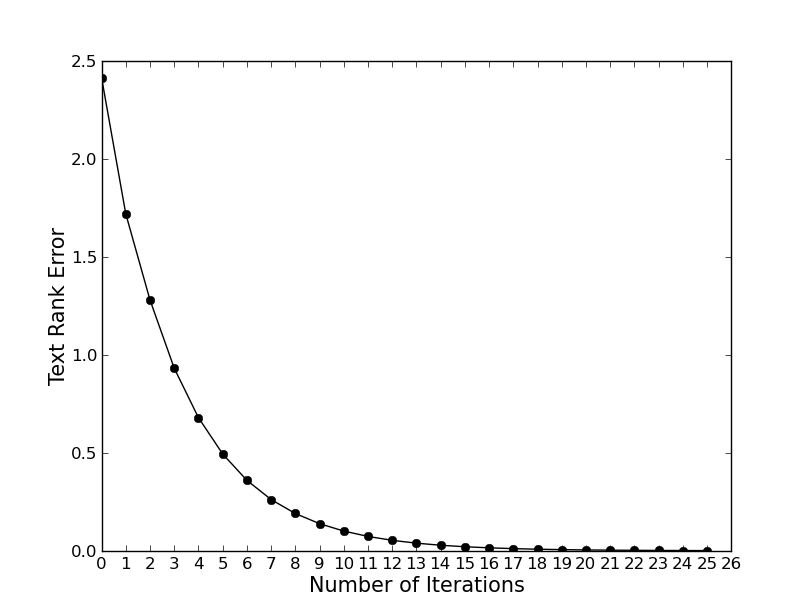
\includegraphics[width=.8\textwidth]{images/error}
    \caption{A plot of Text Rank Error : Error is the sum of magnitudes of score updates performed}
    \label{fig:error}
\end{figure}

\pagebreak
\subsection{First Sentential Overlap}
\emph{First Sentence Overlap} \cite{mead} is defined as the similarity between any sentence in the document and the first sentence in the document.Consider the Docouemt $D$ and $S_1,S_i \in D $, First Sentence Overlap is defined as 
\begin{align}
FSO(S_i) = Similarity(S_i,S_1)
\end{align} 
The First Sentence of a Document is assumed to be it's title. Thus, a sentence with high \emph{First Sentence Overlap} will be talking about the same concept as mentioned in the title and will most likely be coherent with the overall topic of the document.\\

{\noindent \large \underline{Example}} 
\begin{lstlisting}
Tsunami - Death from the seas.
The literal translation of Tsunami is "harbour wave".
A Tsunami is triggered by under water seismic activity.
It is characterized by a series of high waves hitting the coast.
Its lethality is increased because it can strike without warning.
A tsunami can be predicted with underwater seismometers.
Deploying and maintaining them is a challenge.
\end{lstlisting}
The First Sentence Overlap for the above example can be seen in Figure ~\ref{fig:fso}. We can observe that Sentence 2, 3 and 6 get have a high value except for the title.

\begin{figure}[h!]
  \centering
    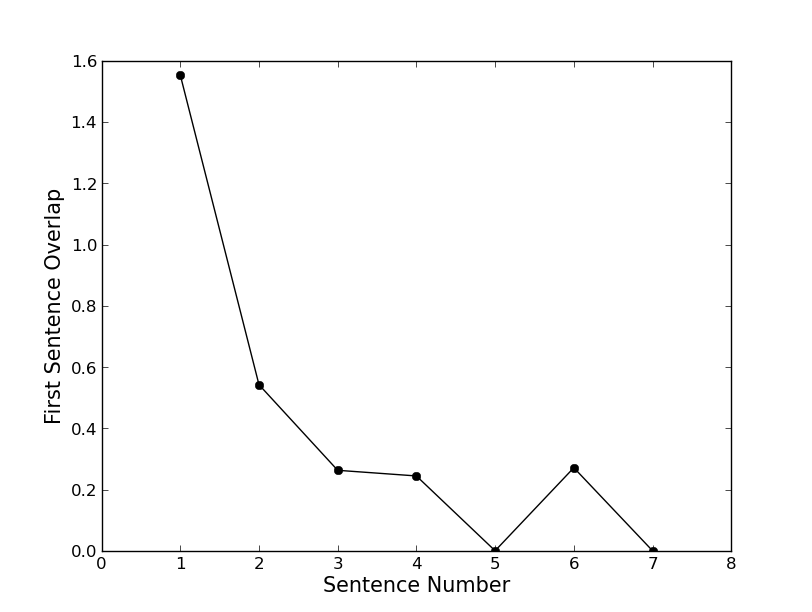
\includegraphics[width=.9\textwidth]{images/fso}
    \caption{A plot of First Sentnence Overlap.}
    \label{fig:fso}
\end{figure}
\pagebreak

\subsection{Gaussian Overlap}
For a Document $D$ and $S_i \in D$
In a document, certain sentences capture the gist of the paragraph. These are likely candidates to be included in the summary. The important property that such sentences share is that they are contain the same words to the preceeding and suceeding sentences. But distant sentences sharing the same words might be relevant. \emph{Gaussian Overlap} considers this similarity and decreases it's significance for farther sentences. For implementation purposes we consider only $-3\sigma$ to $3\sigma$ as statstically significant region of the Gaussian curve.
\begin{align}
GaussianOverlap(S_i) =\sum\limits_{j = - \infty}^{\infty} exp \left( \frac{j}{2\sigma^2} \right) \times Similarity(S_i,S_{i+j})
\end{align}
The Gaussian Overlap values for the above example can be seen in Figure ~\ref{fig:go}. Sentence 7 gets a highhest value because it refers to people.
\newpage

{\noindent \large \underline{Example}} \\
{Document Text ($D_t$)}
\begin{lstlisting}
Human Euthanasia - Good or Evil.
Euthanasia is killing someone, who does not want to live
This is mostly due to their physical misery.
People support euthanasia because they think that it is humane.
It is recommended for patients in a vegetative state.
It improves the quality of life.
It makes economical sense to use the money for other needy people.
People are against euthanasia as they equal it to capital punishment.
It is seen as philosophically flawed and dangerous.
Legalizing it gives to much power to the medical profession.
It can be misused by people to fulfill their bad intentions.
\end{lstlisting}

\begin{figure}[h!]
  \centering
    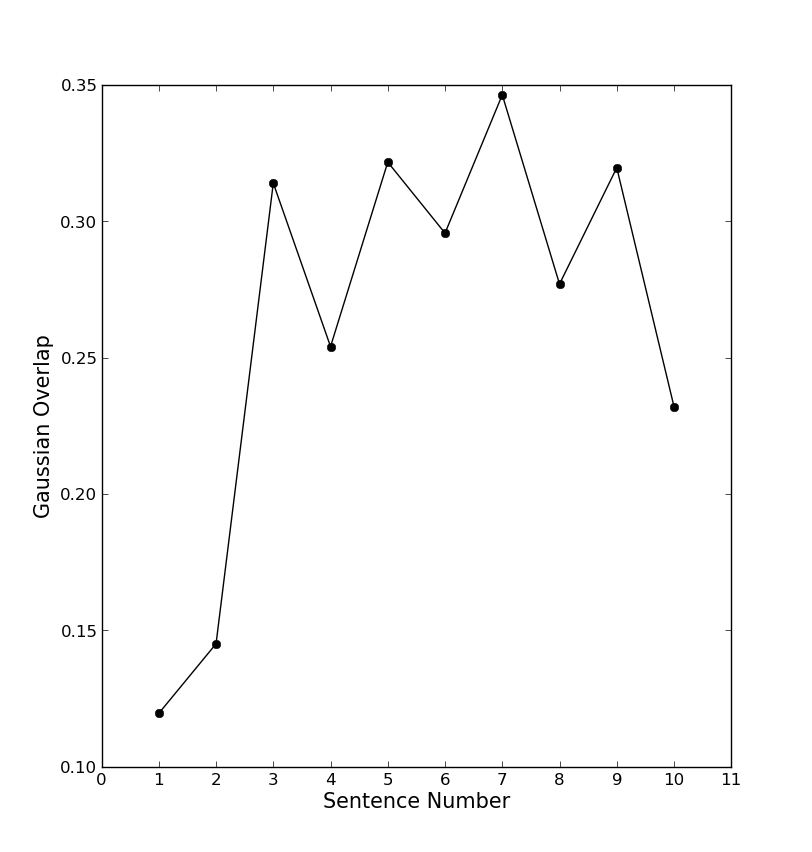
\includegraphics[width=.8\textwidth]{images/go}
    \caption{A plot of Gaussian Overlap }
    \label{fig:go}
\end{figure}
\pagebreak

\section{Importance}
To be able to train our model we need to define how important a sentence in a document is with respect to it's abstractive summary. We need a measure of how much a sentence has contributed to the summary. To do this, we compute the similarity of a sentence in a document with each of the sentences in the summary. We then assign the document sentence an importance score equal to the maximum value of similarity with summary sentences.
\par
Let $D_t$ be the Document representing the document text and $D_s$ be the document representing it's respective summary.\\
For $S_i \in D_t$ 
\begin{align}
Importance(S_i,D_s) = max(\ \{\ Similarity(S_i,S_j)\ |\ S_i \in D_s\ \}\ )  
\end{align}
{\noindent \large \underline{Example}} \\
{Document Text ($D_t$)}
\begin{lstlisting}
Black Holes.
Black holes are regions from which nothing escapes.
They are formed when large stars burn out.
Black holes are incredibly dense.
Hence the escape velocity for objects is very high.
In fact, the escape velocity is faster than the speed of light.
Matter going inside a black hole is lost forever.
They can devour entire planets or stars at a time.
Black holes are found at the centre of all large galaxies.
They are difficult to observe because the do not emit light.
Black holes observed by looking at the light bent by their gravity.
\end{lstlisting}
 \vspace{1.2em}
{Summary Text ($D_s$)}
\begin{lstlisting}
Nothing can escape black holes due to the high escape velocity.
They are formed when stars die out.
They bend the light due to their graivty.
\end{lstlisting}
See Figure ~\ref{fig:importance} for a plot of importance.

\begin{figure}[h!]
  \centering
    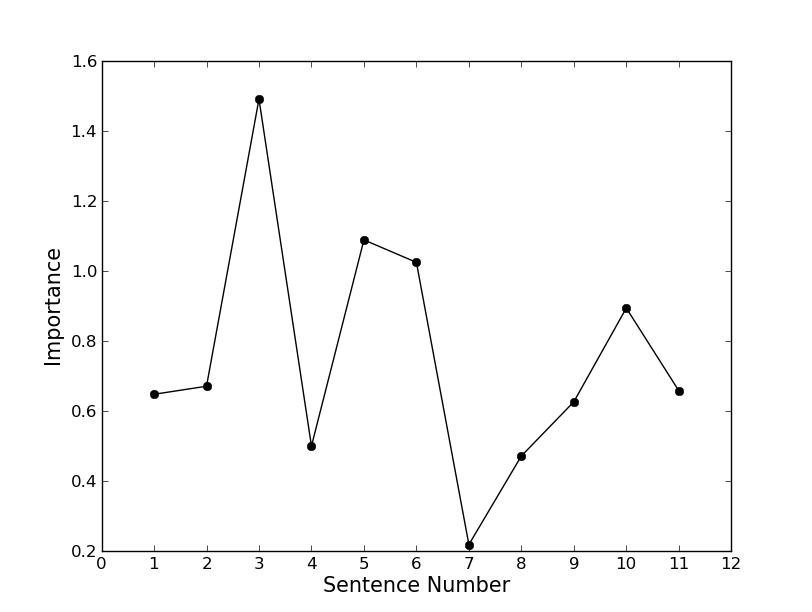
\includegraphics[width=.8\textwidth]{images/importance}
    \caption{A plot of Importance : Notice how Sentence 4,7 and 8 get low importance because the summary doesn't mention density, matter or planets.}
    \label{fig:importance}
\end{figure}

\chapter{Results}
The proposed method was implemented in Python, using scikit-learn\cite{sklearn} for Support Vector Regression. The source code for our implementation is available on github\cite{code}.
To evaluate our system, we took three documents of different categories (a news article, a technical document and a movie review) and generated abstractive summaries for them, which were used for training. Three more documents, one of each of the above types, were taken and summarized using the trained system. These summaries were evaluated against three human generated summaries using ROUGE scores, out of which the F-Score parameter was considered. The results are available in the following table:\\
\\
\begin{tabular}{|l||*{3}{c|}}\hline
\backslashbox{ \small{Training Article}\\ \small{Category} }{\small{Article}\\ \small{Category}}
&\makebox[3em]{Review}&\makebox[3em]{Technical}&\makebox[3em]{News}\\\hline\hline
Review &0.31579&0.16988&.26866\\\hline
Technical &0.35065&.16000&.30769\\\hline
News &0.22951&0.16217&0.26866\\\hline
\end{tabular}\\
\par
In the above table, we observe that training against news and review articles gives us better summaries for news and review articles respectively. Technical articles don't exhibit such an analogy. This might be due to that fact that technical articles are already concise and omitting sentences might result in an information loss. Also the features we have used might be inapproporiate to capture certain global properties of sentences.
%%%%%%%%%%%%%%%%%%%%%%%%%%%%%%%%%%%%%%%%%%%%%%%%%%%%%%%%%%%%
% Bibliography.

\chapter{Conclusion}
We have modelled Extractive Summarization as a Machine Learning problem. We used Abstractive Summaries to train our model. We used the model so trained to predict significance of sentences to select them for an Extractive summary. Our model is likely to better summarize articles of the same type that it is trained with. The features we have used are limited in terms of their number and scope. Better features may be used in the future to better summarize various kinds of documents. Since we are comparing words as they are, comparing words in their root forms might yield better results.
\begin{singlespace}
  \bibliography{report}
\end{singlespace}

\chapter{Appendix A: Training Documents}
\section{Training Documents}

\subsubsection{Infamous Second Son (Review)}
\begin{lstlisting}[basicstyle=\scriptsize]
Seattle is a police state.
Department of Unified Protection director Brooke Augustine has set her fascist government organization loose on the God-fearing populace, abusing her power to round up those with mutant abilities.
Unmanned drones patrol the skies, invasive checkpoints detain suspected bio-terrorists, and high-tech surveillance cameras monitor everyone's actions.
It's a city built upon fear.
The citizens willingly accept their new overlords because so many are scared of their friends and neighbors who are now imbued with superpowers.
So when protagonist Delsin Rowe finds that he is able to absorb others' powers, he enters a society ready to pour their hatred upon him.
Do you fight those who loathe you? Or free Seattle from the chains of an oppressive dictatorship?
The world of Infamous: Second Son plays upon the recent changes that have taken place within our own society.
By offering an exaggerated viewpoint of the safety-over-freedom measures that are now a part of our daily lives, we see how dangerous such a path could be, and how few people rise up if their lives remain comfortable.
It's an intriguing setup, but one that fails to stir a strong emotional response.
The binary morality doesn't show a balanced angle that could have made you sympathize with the government's actions, even if you disagree with how those rules are enacted, and that one-sided viewpoint turns what should be a hard-hitting situation into one that's difficult to relate to.
You see the situation through the eyes of Delsin.
His youth was spent spray painting cartoonish doodles while avoiding the wrath of his older brother, Reggie, a police officer with a firm belief in what's right and what's illegal.
Delsin's immaturity is immediately an annoyance as he spouts terrible one-liners while shirking any responsibility.
During the first hour of Second Son, you're stuck watching cutscene after cutscene establish the fiction, and that uneven pacing feels like shackles preventing you from exploring this gorgeous world.
However, once you're set loose in Seattle, the narrative problems that haunted the early moments fade into the background as you flex your elemental muscles.
Delsin has a run-in with the escaped conduit Hank, who has smoke coursing through his veins.
That chance meeting transforms Delsin from just another forgotten screw-up into the potential savior of a beautiful metropolis.
Through the power of smoke, you can turn into a translucent wisp at a moment's notice.
Float through air vents to propel yourself from the rain-drenched streets to the striking rooftops or drift like an ethereal shadow among the citizens compelled to fear you.
The empowering sense of freedom worms its way into your heart once you realize your unbelievable potential.
The slow-paced, methodical movement that defined the two earlier Infamous games has been stripped away here, replaced by a frenetic speed that has you rushing through this open world like a sentient lightning bolt.
Fights are structured for you to take advantage of your extraordinary abilities.
Snipers perch upon billboards, armored vans carry reinforcements, and helicopters patrol the skies.
Troops have the power of cement to complement their standard arsenal.
They construct concrete walls and dive upon you with deadly might, so standing still is an easy way for you to meet a quick end.
So you show off your quick feet, drifting into and out of fights, peppering aggressors with flaming missiles while you dance just out of their deadly strikes.
Take too much damage, and your view becomes oversaturated while an angelic voice scores the soundtrack of your death.
Unlike in previous Infamous games, your health regenerates over time, so knowing when to seek shelter and when to stay aggressive forces you to fight thoughtfully.
Second Son has a binary morality system that mirrors the black-and-white decision making from the previous games.
If you're a callous jerk, for instance, you can choose to forsake your Native American heritage to avoid punitive measures from Augustine.
If you'd rather sleep with a sound conscience, take responsibility for your actions so your tribe doesn't suffer.
Without a moral gray area, these choices filter reality through a cartoonish prism where only pure good and unadulterated evil exist.
Though these extreme decisions feel totally disconnected from reality, the manner in which this dichotomy exists within the framework of combat adds serious weight to your every action.
Delsin earns a single-use, screen-clearing attack no matter which side of the morality coin you fall on.
When you play as a hero, you must tread with a light touch.
You need to subdue enemies with smoke handcuffs instead of killing them off, and make sure you direct your attacks away from ordinary citizens.
If you fail to follow these basic rules, your chain breaks, and your chance to use your most powerful attack disappears.
On the villainous side, chaos is the key to earning that most treasured of prizes.
Not only must you kill every attacker, but you must do so as quickly as possible.
If you spend too much time between conquests, your multiplier vanishes, so you must act as aggressively as possible, indiscriminately exterminating anyone who moves.
Such opposing play styles better communicated who my Delsin was than the many tired cutscenes that encompass the rest of the narrative.
During my first playthrough, I was as good as possible, so I fought with a methodical, thoughtful air that made me consider each flaming missile that I lobbed.
I used restraint.
When my health diminished, I hid in the shadows so as not to succumb to the angry forces.
After a hectic victory, I would look upon the battlefield with wry satisfaction.
My enemies lay prone before me, chained to the ground, left to think about the path they had chosen.
I was both victorious and righteous.
The citizenry recognized my efforts, and celebrated me when I walked the streets.
I was a hero in action and word, and their fears of the unknown slowly dissipated.
It was during my second time through that I took the evil route and realized the extent of my extraordinary powers.
No longer did I hold back.
When an armored van would arrive, I would immediately toss missiles toward it, unconcerned about the collateral damage that would result.
Overwhelmed enemies would surrender, desperate for respite, and as they walked toward me with arms raised above their heads, I would maniacally laugh as I lit their heads on fire.
When bullets pierced me from every direction, I would grow angry, becoming even more reckless as I desperately tried to fill my kill quota.
No one was safe when my Delsin was around.
And the citizens who were taught to fear me yelled hateful remarks as I walked through the streets.
The dumb ones, at least.
I killed my share of loose-lipped normals.
Combat strikes a happy balance between the slow-paced affairs of the first Infamous and the overly chaotic endeavors of Infamous 2.
Second Son offers speed with a purpose.
So fine-tuned are your actions that you move with blinding speed and yet are always aware of your surroundings.
Ensuring the action stays hectic without becoming overbearing is an extraordinary accomplishment, so much so that I happily played through twice only to still remain hungry for more.
As I sprinted up the sides of buildings and called in explosive strikes, Second Son felt less like another Infamous and more like a new entry in the Prototype franchise.
It's so fast, so frenetic, and so gloriously over the top that it makes the old days of Cole McGrath slowly climbing buildings seem like a distant memory.
Delsin gains access to more powers beyond the smoke you start off with, and each transforms both the action and locomotion in interesting ways.
You might employ a slow-motion effect to corral your enemies in a precise manner, or mix stealth into your explosive encounters to keep enemies guessing, and such twists ensure that each showdown keeps you thinking up new tactics as you revel in the destructive glory.
Sadly, the powers don't branch in interesting ways depending on your moral choices, so though combat plays out in different ways, the weapons you use are nearly identical.
Missions present scenarios that urge you to fight in inventive ways.
The myriad ways in which you flex your combat prowess left me glued to the screen as I eagerly overcame every roadblock in my way.
Bosses mirror the brilliance of the normal forays by compelling you to move with speed and precision as you mount a hellacious counterattack.
Fights stretch on longer than I expected, but instead of being tedious wars of attrition, they instead kept me riveted as I tried to perfect my craft.
Standing up to my overpowered foes for these long battles felt like a victory well earned, and I was happy with the assortment of bosses on offer through the course of this adventure.
Second Son has top-notch combat that expertly melds substance with style.
But despite the speed that separates this from previous games in the franchise, there's a feeling of familiarity that's impossible to shake.
The Seattle in Second Son offers a stark contrast to the direction recent open-world games have taken.
This is not a living, breathing world that you inhabit.
Rather, it's a playground for you to go nuts in.
The people who populate the world exist only for your benefit, so it never feels like a real city.
It's an anachronistic return to what sandbox games used to be, and represents an approach that I still enjoy more than the serious options that populate store shelves.
Still, I couldn't help yearning for more concrete improvements to what I've already experienced.
The cutting-edge visuals are laid over a decade-old formula that is still fun though sadly showing its age.
That certainly didn't prevent me from getting 100 percent on both a good and an evil playthrough.
Side missions nicely complement your story efforts so you have plenty of reason to roam if you want to spend more time in pristine Seattle.
Second Son is not the tedious collect-a-thon that many open-world games are.
Extra activities are clearly labeled on the map, so instead of wandering aimlessly around the rainy streets, you focus on maximizing your enjoyment.
My favorite detour was spray painting inspiring messages on walls.
Sure, the act of tilting the motion-enabled controller at the stencils was hardly thrilling, but seeing what artistic propaganda Delsin cooked up was always a treat.
Creating graffiti isn't the only way an unusual control scheme is used.
During context-sensitive situations, you must manipulate the touchpad, and though this sounds incredibly gimmicky, it actually added to my immersion.
Swiping to open a door to free those suspected of being conduits engaged me more than pushing a button could, as did holding my thumbs firmly on the pad as Delsin grabbed a generator he was trying to destroy.
Employing controls different from the norm is always a tricky endeavor, and Sucker Punch did a great job of ensuring these little moments added to the experience rather than distracting from your actions.
Second Son focuses on pure enjoyment.
It communicates that through the excellent combat that forces you to concoct crazy tactics to overthrow the invading forces.
It draws you in further through its incredible visuals that not only hint at the PlayStation 4's impressive power, but employ a sensible artistic touch that makes Seattle a place you want to explore.
It uses a complementary score to underline dramatic moments, and the sound effects pop with flair.
And yet, for all of the elements in which Second Son excels, the narrative fails to carry its share of the weight.
Still, don't become mired in the negativity as Delsin so often does.
Instead, just laugh at the cheesy dialogue and chortle at how extreme the morality system is.
Second Son is a great game that knows exactly what it is, and sucks you in with its unfiltered fun.
\end{lstlisting}

\subsubsection{End of Windows XP: Who all are at risk (News)}
\begin{lstlisting}[basicstyle=\scriptsize]
Microsoft will end support for the persistently popular Windows XP on Tuesday, and the move could put everything from the operations of heavy industry to the identities of everyday people in danger.
An estimated 30% of computers being used by businesses and consumers around the world are still running the 12-year-old operating system.
"What once was considered low-hanging fruit by hackers now has a big neon bull's eye on it," says Patrick Thomas, a security consultant at the San Jose, California-based firm Neohapsis.
Microsoft has released a handful of Windows operating systems since 2001, but XP's popularity and the durability of the computers it was installed on kept it around longer than expected. Analysts say that if a PC is more than five years old, chances are it's running XP.
While users can still run XP after Tuesday, Microsoft says it will no longer provide security updates, issue fixes to non-security related problems or offer online technical content updates. The company is discontinuing XP to focus on maintaining its newer operating systems, the core programs that run personal computers.
The Redmond, Washington-based company says it will provide anti-malware-related updates through July 14, 2015, but warns that the tweaks could be of limited help on an outdated operating system.
Most industry experts say they recognize that the time for Microsoft to end support for such a dated system has come, but the move poses both security and operational risks for the remaining users. In addition to home computers, XP is used to run everything from water treatment facilities and power plants to small businesses like doctor's offices.
Thomas says XP appealed to a wide variety of people and businesses that saw it as a reliable workhorse and many chose to stick with it instead of upgrading to Windows Vista, Windows 7 or 8.
Thomas notes that companies generally resist change because they don't like risk. As a result, businesses most likely to still be using XP include banks and financial services companies, along with health care providers. He also pointed to schools from the university level down, saying that they often don't have enough money to fund equipment upgrades.
Marcin Kleczynski, CEO of Malwarebytes, says that without patches to fix bugs in the software XP PCs will be prone to freezing up and crashing, while the absence of updated security related protections make the computers susceptible to hackers.
He added that future security patches released for Microsoft's newer systems will serve as a way for hackers to reverse engineer ways to breach now-unprotected Windows XP computers.
"It's going to be interesting to say the least," he says. "There are plenty of black hats out there that are looking for the first vulnerability and will be looking at Windows 7 and 8 to find those vulnerabilities. And if you're able to find a vulnerability in XP, it's pretty much a silver key."
Those weaknesses can affect businesses both large and small.
Mark Bernardo, general manager of automation software at General Electric's Intelligent Platforms division, says moving to a new operating system can be extremely complicated and expensive for industrial companies. Bernardo, whose GE division offers advisory services for upgrading from XP, says many of the unit's customers fall into the fields of water and waste water, along with oil and gas.
"Even if their sole network is completely sealed off from attack, there are still operational issues to deal with," he says.
Meanwhile, many small businesses are put off by the hefty cost of upgrading or just aren't focused on their IT needs. Although a consumer can buy an entry-level PC for a few hundred dollars, a computer powerful enough for business use may run $1,000 or more after adding the necessary software.
Barry Maher, a salesperson trainer and motivational speaker based in Corona, Calif., says his IT consultant warned him about the end of XP support last year. But he was so busy with other things that he didn't start actively looking for a new computer until a few weeks ago.
"This probably hasn't been as high a priority as it should have been," he says.
He got his current PC just before Microsoft released Vista in 2007. He never bought another PC because, "As long as the machine is doing what I want it to do, and running the software I need to run, I would never change it."
Mark McCreary, a Philadelphia-based attorney with the firm Fox Rothschild LLP, says small businesses could be among the most effected by the end of support, because they don't have the same kinds of firewalls and in-house IT departments that larger companies possess. And if they don't upgrade and something bad happens, they could face lawsuits from customers.
But he says he doesn't expect the wide-spread malware attacks and disasters that others are predicting - at least for a while.
"It's not that you blow it off and wait another seven years, but it's not like everything is going to explode on April 8 either," he says.
McCreary points to Microsoft's plans to keep providing malware-related updates for well over a year, adding that he doubts hackers are actually saving up their malware attacks for the day support ends.
But Sam Glines, CEO of Norse, a threat-detection firm with major offices in St Louis and Silicon Valley, disagrees. He believes hackers have been watching potential targets for some time now.
"There's a gearing up on the part of the dark side to take advantage of this end of support," Glines says.
He worries most about doctors like his father and others the health care industry, who may be very smart people, but just aren't focused on technology. He notes that health care-related information is 10 to 20 times more valuable on the black market than financial information, because it can be used to create fraudulent medical claims and illegally obtain prescription drugs, making doctor's offices tempting targets.
Meanwhile, without updates from Microsoft, regular people who currently use XP at home need to be extra careful.
Mike Eldridge, 39, of Spring Lake, Mich, says that since his computer is currently on its last legs, he's going to cross his fingers and hope for the best until it finally dies.
"I am worried about security threats, but I'd rather have my identity stolen than put up with Windows 8," he says.
\end{lstlisting}

\subsubsection{Big Data (Technical)}
\begin{lstlisting}[basicstyle=\scriptsize]
Big data is the term for a collection of data sets so large and complex that it becomes difficult to process using on-hand database management tools or traditional data processing applications.
The challenges include capture, curation, storage, search, sharing, transfer, analysis and visualization.
The trend to larger data sets is due to the additional information derivable from analysis of a single large set of related data, as compared to separate smaller sets with the same total amount of data, allowing correlations to be found to "spot business trends, determine quality of research, prevent diseases, link legal citations, combat crime, and determine real-time roadway traffic conditions."
As of 2012, limits on the size of data sets that are feasible to process in a reasonable amount of time were on the order of exabytes of data.
Scientists regularly encounter limitations due to large data sets in many areas, including meteorology, genomics, connectomics, complex physics simulations, and biological and environmental research. 
The limitations also affect Internet search, finance and business informatics.
Data sets grow in size in part because they are increasingly being gathered by ubiquitous information-sensing mobile devices, aerial sensory technologies (remote sensing), software logs, cameras, microphones, radio-frequency identification readers, and wireless sensor networks.
The world's technological per-capita capacity to store information has roughly doubled every 40 months since the 1980s; as of 2012, every day 2.5 exabytes (2.5×1018) of data were created.
The challenge for large enterprises is determining who should own big data initiatives that straddle the entire organization.
Big data is difficult to work with using most relational database management systems and desktop statistics and visualization packages, requiring instead "massively parallel software running on tens, hundreds, or even thousands of servers".
What is considered "big data" varies depending on the capabilities of the organization managing the set, and on the capabilities of the applications that are traditionally used to process and analyze the data set in its domain.
"For some organizations, facing hundreds of gigabytes of data for the first time may trigger a need to reconsider data management options.
For others, it may take tens or hundreds of terabytes before data size becomes a significant consideration."
\end{lstlisting}
\pagebreak
\section{Test Documents}
\subsubsection{300: Rise Of An Empire (Review)}
\begin{lstlisting}[basicstyle=\scriptsize]
The invading Persian forces led by the god-like Xerxes and navy commander Artemisia battle the Greeks (led by Themistocles) in the hope of conquering the land.
With the odds against him, Themistocles must use guile and strength in equal measure to save Greece from destruction. 
Review: While the first 300 movie dealt with Leonidas and the events at Thermopylae, here the focus shifts to the equally furious sea battle, fought on dark, choppy waters.
King Xerxes (Santoro) and Queen Gorgo of Sparta (Headey) face off, with their respective commanders Artemisia (Green) and Themistocles (Stapleton) leading their navies. Although the previous movie is referenced in the gorgeous opening shot, the battle then rides on Themistocles' able shoulders.
Artemisia is a determined commander, who doesn't think much of her adversaries, clad in sandals and capes. Indeed, the Persian navy splinters the Greek galleys, until they come up against Themistocles.
Artemisia realises that she has an equal in strategy and cunning, against whom overwhelming force and superior numbers alone won't work.
Themistocles, although lacking the crazed blood-lust that drove Leonidas, is weary of war. Yet, he knows that each of them would have to, if need be, make the ultimate sacrifice to save 'Mother Greece'.
He shows his resolve when mustering the Greek forces with lines like, "We choose to die on our feet rather than live on our knees!" But is he immune to Artemisia's female charms or will those prove to be his Achilles heel?
Xerxes himself, looking like he has emerged from a gold bath and resplendent in various piercings, is relegated to a few booming sentences.
The blood and gore is off the scale; warriors are hacked and cleaved in glorious CGI detail.
Part-vamp and part-warrior princess in leather, Green is stunning as Artemisia. The film itself looks fantastic, awash in a red-sepia tone that dominates everything.
Although you will have seen many action films set during a point of time in history (this one's set in 480 BC), there is plenty in here to keep your attention from start to finish.
\end{lstlisting}

\subsubsection{Pakistani actress Sana Khan dies in road accident (News)}
\begin{lstlisting}[basicstyle=\scriptsize]
Pakistani actress Sana Khan has died in an accident near Looni Kot, around 30 km off Hyderabad, a media report said.
Sana and her husband actor Babar Khan were on their way from Karachi to Hyderabad in a car when the vehicle, driven by Babar, went out of control Friday, reports dawn.com.
The car overturned, leaving the duo seriously injured.
The motorway police and ambulance reached the spot soon after receiving the information, and shifted them to Liaquat University Hospital Jamshoro.
Sana breathed her last before she could get any first aid while Babar was later shifted to Liaquat University Hospital City Branch.
Babar, who had married Sana in December 2013, is said to be in critical condition.
Sana was known for her appearance in a serial "Parchaiyan" and Babar is known for the serial "Ek Tamana Lahasil Se".
\end{lstlisting}

\subsubsection{Abstractions in Programming Languages (Technical)}
\begin{lstlisting}[basicstyle=\scriptsize]
Abstractions in programming languages.
All programming languages provide abstractions.
It can be argued that the complexity of the problems you're able to solve is directly related to the kind and quality of abstraction.
By "kind" I mean, "What is it that you are abstracting?".
Assembly language is a small abstraction of the underlying machine.
Many so-called "imperative" languages that followed (such as Fortran, BASIC, and C) were abstractions of assembly language.
These languages are big improvements over assembly language, but their primary abstraction still requires you to think in terms of the structure of the computer rather than the structure of the problem you are trying to solve.
The programmer must establish the association between the machine model (in the "solution space," which is the place where you're modeling that problem, such as a computer) and the model of the problem that is actually being solved (in the "problem space," which is the place where the problem exists).
The effort required to perform this mapping, and the fact that it is extrinsic to the programming language, produces programs that are difficult to write and expensive to maintain, and as a side effect created the entire "programming methods" industry.
The alternative to modeling the machine is to model the problem you're trying to solve.
Early languages such as LISP and APL chose particular views of the world ("All problems are ultimately lists" or "All problems are algorithmic").
PROLOG casts all problems into chains of decisions. 
Languages have been created for constraint-based programming and for programming exclusively by manipulating graphical symbols (the latter proved to be too restrictive).
Each of these approaches is a good solution to the particular class of problem they're designed to solve, but when you step outside of that domain they become awkward.
The object-oriented approach goes a step farther by providing tools for the programmer to represent elements in the problem space.
This representation is general enough that the programmer is not constrained to any particular type of problem.
We refer to the elements in the problem space and their representations in the solution space as "objects" (of course, you will also need other objects that don't have problem-space analogs).
The idea is that the program is allowed to adapt itself to the lingo of the problem by adding new types of objects, so when you read the code describing the solution, you're reading words that also express the problem.
This is a more flexible and powerful language abstraction than what we've had before.
Thus, OOP allows you to describe the problem in terms of the problem, rather than in terms of the computer where the solution will run. 
There's still a connection back to the computer, though.
Each object looks quite a bit like a little computer; it has a state, and it has operations that you can ask it to perform.
However, this doesn't seem like such a bad analogy to objects in the real world; they all have characteristics and behaviors.
Some language designers have decided that object-oriented programming by itself is not adequate to easily solve all programming problems, and advocate the combination of various approaches into multiparadigm programming languages.
\end{lstlisting}

\chapter{Appendix B: Summaries}
\section{Summary When Trained Against the Review Article}
\subsubsection{300: Rise of an empire}
\begin{lstlisting}[basicstyle=\scriptsize]
The invading Persian forces led by the god-like Xerxes and navy commander Artemisia battle the Greeks (led by Themistocles) in the hope of conquering the land.
Review: While the first 300 movie dealt with Leonidas and the events at Thermopylae, here the focus shifts to the equally furious sea battle, fought on dark, choppy waters.
Although you will have seen many action films set during a point of time in history (this one's set in 480 BC), there is plenty in here to keep your attention from start to finish.
\end{lstlisting}
\subsubsection{Abstractions in Programming Languages}
\begin{lstlisting}[basicstyle=\scriptsize]
It can be argued that the complexity of the problems you're able to solve is directly related to the kind and quality of abstraction.
These languages are big improvements over assembly language, but their primary abstraction still requires you to think in terms of the structure of the computer rather than the structure of the problem you are trying to solve.
The programmer must establish the association between the machine model (in the "solution space," which is the place where you're modeling that problem, such as a computer) and the model of the problem that is actually being solved (in the "problem space," which is the place where the problem exists).
The effort required to perform this mapping, and the fact that it is extrinsic to the programming language, produces programs that are difficult to write and expensive to maintain, and as a side effect created the entire "programming methods" industry.
The idea is that the program is allowed to adapt itself to the lingo of the problem by adding new types of objects, so when you read the code describing the solution, you're reading words that also express the problem.
\end{lstlisting}
\subsubsection{Pakistani actress Sana Khan dies in road Accident}
\begin{lstlisting}[basicstyle=\scriptsize]
Sana and her husband actor Babar Khan were on their way from Karachi to Hyderabad in a car when the vehicle, driven by Babar, went out of control Friday, reports dawn.
\end{lstlisting}
\section{Summary When Trained Against the News Article}
\subsubsection{300: Rise of an empire}
\begin{lstlisting}[basicstyle=\scriptsize]
Although the previous movie is referenced in the gorgeous opening shot, the battle then rides on Themistocles' able shoulders.
Indeed, the Persian navy splinters the Greek galleys, until they come up against Themistocles.
The blood and gore is off the scale; warriors are hacked and cleaved in glorious CGI detail.
\end{lstlisting}
\subsubsection{Abstractions in Programming Languages}
\begin{lstlisting}[basicstyle=\scriptsize]
These languages are big improvements over assembly language, but their primary abstraction still requires you to think in terms of the structure of the computer rather than the structure of the problem you are trying to solve.
The programmer must establish the association between the machine model (in the "solution space," which is the place where you're modeling that problem, such as a computer) and the model of the problem that is actually being solved (in the "problem space," which is the place where the problem exists).
The effort required to perform this mapping, and the fact that it is extrinsic to the programming language, produces programs that are difficult to write and expensive to maintain, and as a side effect created the entire "programming methods" industry.
The idea is that the program is allowed to adapt itself to the lingo of the problem by adding new types of objects, so when you read the code describing the solution, you're reading words that also express the problem.
Thus, OOP allows you to describe the problem in terms of the problem, rather than in terms of the computer where the solution will run.
\end{lstlisting}
\subsubsection{Pakistani actress Sana Khan dies in road Accident}
\begin{lstlisting}[basicstyle=\scriptsize]
Sana and her husband actor Babar Khan were on their way from Karachi to Hyderabad in a car when the vehicle, driven by Babar, went out of control Friday, reports dawn.
\end{lstlisting}
\section{Summary When Trained Against the Technical Article}
\subsubsection{300: Rise of an empire}
\begin{lstlisting}[basicstyle=\scriptsize]
300: Rise Of An Empire (Review)  Story: The invading Persian forces led by the god-like Xerxes and navy commander Artemisia battle the Greeks (led by Themistocles) in the hope of conquering the land.
Review: While the first 300 movie dealt with Leonidas and the events at Thermopylae, here the focus shifts to the equally furious sea battle, fought on dark, choppy waters.
Although the previous movie is referenced in the gorgeous opening shot, the battle then rides on Themistocles' able shoulders.
\end{lstlisting}
\subsubsection{Abstractions in Programming Languages}
\begin{lstlisting}[basicstyle=\scriptsize]
These languages are big improvements over assembly language, but their primary abstraction still requires you to think in terms of the structure of the computer rather than the structure of the problem you are trying to solve.
The programmer must establish the association between the machine model (in the "solution space," which is the place where you're modeling that problem, such as a computer) and the model of the problem that is actually being solved (in the "problem space," which is the place where the problem exists).
The effort required to perform this mapping, and the fact that it is extrinsic to the programming language, produces programs that are difficult to write and expensive to maintain, and as a side effect created the entire "programming methods" industry.
The alternative to modeling the machine is to model the problem you're trying to solve.
The idea is that the program is allowed to adapt itself to the lingo of the problem by adding new types of objects, so when you read the code describing the solution, you're reading words that also express the problem.
\end{lstlisting}
\subsubsection{Pakistani actress Sana Khan dies in road Accident}
\begin{lstlisting}[basicstyle=\scriptsize]
Pakistani actress Sana Khan dies in road accident  Pakistani actress Sana Khan has died in an accident near Looni Kot, around 30 km off Hyderabad, a media report said.
\end{lstlisting}
%%%%%%%%%%%%%%%%%%%%%%%%%%%%%%%%%%%%%%%%%%%%%%%%%%%%%%%%%%%%
% List of papers

% \listofpapers

% \begin{enumerate}  
% \item Authors....  \newblock
%  Title...
%   \newblock {\em Journal}, Volume,
%   Page, (year).
% \end{enumerate}  

\end{document}
	